%% LyX 2.1.3 created this file.  For more info, see http://www.lyx.org/.
%% Do not edit unless you really know what you are doing.
\documentclass{article}\usepackage[]{graphicx}\usepackage[]{color}
%% maxwidth is the original width if it is less than linewidth
%% otherwise use linewidth (to make sure the graphics do not exceed the margin)
\makeatletter
\def\maxwidth{ %
  \ifdim\Gin@nat@width>\linewidth
    \linewidth
  \else
    \Gin@nat@width
  \fi
}
\makeatother

\definecolor{fgcolor}{rgb}{0.345, 0.345, 0.345}
\newcommand{\hlnum}[1]{\textcolor[rgb]{0.686,0.059,0.569}{#1}}%
\newcommand{\hlstr}[1]{\textcolor[rgb]{0.192,0.494,0.8}{#1}}%
\newcommand{\hlcom}[1]{\textcolor[rgb]{0.678,0.584,0.686}{\textit{#1}}}%
\newcommand{\hlopt}[1]{\textcolor[rgb]{0,0,0}{#1}}%
\newcommand{\hlstd}[1]{\textcolor[rgb]{0.345,0.345,0.345}{#1}}%
\newcommand{\hlkwa}[1]{\textcolor[rgb]{0.161,0.373,0.58}{\textbf{#1}}}%
\newcommand{\hlkwb}[1]{\textcolor[rgb]{0.69,0.353,0.396}{#1}}%
\newcommand{\hlkwc}[1]{\textcolor[rgb]{0.333,0.667,0.333}{#1}}%
\newcommand{\hlkwd}[1]{\textcolor[rgb]{0.737,0.353,0.396}{\textbf{#1}}}%

\usepackage{framed}
\makeatletter
\newenvironment{kframe}{%
 \def\at@end@of@kframe{}%
 \ifinner\ifhmode%
  \def\at@end@of@kframe{\end{minipage}}%
  \begin{minipage}{\columnwidth}%
 \fi\fi%
 \def\FrameCommand##1{\hskip\@totalleftmargin \hskip-\fboxsep
 \colorbox{shadecolor}{##1}\hskip-\fboxsep
     % There is no \\@totalrightmargin, so:
     \hskip-\linewidth \hskip-\@totalleftmargin \hskip\columnwidth}%
 \MakeFramed {\advance\hsize-\width
   \@totalleftmargin\z@ \linewidth\hsize
   \@setminipage}}%
 {\par\unskip\endMakeFramed%
 \at@end@of@kframe}
\makeatother

\definecolor{shadecolor}{rgb}{.97, .97, .97}
\definecolor{messagecolor}{rgb}{0, 0, 0}
\definecolor{warningcolor}{rgb}{1, 0, 1}
\definecolor{errorcolor}{rgb}{1, 0, 0}
\newenvironment{knitrout}{}{} % an empty environment to be redefined in TeX

\usepackage{alltt} 
\usepackage{ucs}
\usepackage[utf8x]{inputenc}
\usepackage[sc]{mathpazo}
\usepackage[T1]{fontenc}
\usepackage{geometry}

\newenvironment{uzdevums}[1][\unskip]{%
\vspace{3mm}
\noindent
\textbf{#1 uzdevums:}
\noindent}
{}

\geometry{verbose,tmargin=2.5cm,bmargin=2.5cm,lmargin=2.5cm,rmargin=2.5cm}
\setcounter{secnumdepth}{2}
\setcounter{tocdepth}{2}
\usepackage{url}
\usepackage[unicode=true,pdfusetitle,
 bookmarks=true,bookmarksnumbered=true,bookmarksopen=true,bookmarksopenlevel=2,
 breaklinks=false,pdfborder={0 0 1},backref=false,colorlinks=false]
 {hyperref}
\renewcommand{\abstractname}{Anotācija}
\hypersetup{
 pdfstartview={XYZ null null 1}}
\IfFileExists{upquote.sty}{\usepackage{upquote}}{}
\begin{document}



\title{41.\ AMO rezultāti tabulās un zīmējumos}

\author{}
\date{}

\maketitle

\begin{abstract}
Šajā dokumentā apkopoti daži 41.\ Atklātās matemātikas olimpiādes (2014.m.g.) rezultātu kop\-sa\-vil\-ku\-mi. Izmantojot izklājlapas, ko publisko LU Neklātienes Matemātikas Skola, aprēķināts dalībnieku skaits, dalības aktivitāte (AMO dalībnieku īpatsvars no visiem attiecīgā vecuma skolēniem), dalība un rezultāti atkarībā no skolēnu \v{g}eogrāfijas, urbanizācijas, valodas, dzimuma. Apkopoti saraksti ar skolotājiem un skolām, kas nodrošinājuši augstu dalību vai ieguvuši lielu punktu kopskaitu. Pārskata nobeigumā minēti dati arī par uzdevumiem --- vidējais punktu skaits un vērtējumu sadalījums, kāda daļa no rēķinātājiem neuzsāka risināt (``mīnusu'' jeb neatrasto risinājumu skaits galavērtējumā), kāda ir konkrētā uzdevuma vērtējumu korelācija ar pārējo uzdevumu vērtējumu summu. 
\end{abstract}

\section{Dalībnieku aktivitāte}

Šajā sadaļā atbildēsim uz jautājumu, kāda daļa no 6.klasei atbilstošās vecuma grupas skolēniem piedalījās 42.\ AMO. 
Dati par skolēnu skaitu pa re\v{g}ioniem, klasēm un mācību valodām ņemti no IZM publiskotās statistikas --- \url{http://izm.gov.lv/lv/publikacijas-un-statistika/statistika-par-visparejo-izglitibu/2014-2015-m-g}. Dati apkopoti par 9 lielajām pilsētām kā arī par re\v{g}ioniem, kuros nav ietvertas lielās pilsētas. Ar {\em re\v{g}ioniem} domāti NUTS 3 re\v{g}ioni --- sk. \url{http://en.wikipedia.org/wiki/Statistical_regions_of_Latvia} - Kurzeme, Latgale, Pierīga Rīga, Vidzeme, Zemgale.


\subsection{Dalība olimpiādē}



%% col1 = region
%% col2 = participants
%% col3 = total guys
%% col4 = percentage participated

\begin{knitrout}
\definecolor{shadecolor}{rgb}{0.969, 0.969, 0.969}\color{fgcolor}
\begin{tabular}{l|r|r|r}
\hline
  & Participants & All (Grades 5-12) & Activity\\
\hline
Liepaja & 48 & 4863 & 0.99\\
\hline
Ventspils & 46 & 2456 & 1.87\\
\hline
Cita Kurzeme & 95 & 9371 & 1.01\\
\hline
Daugavpils & 150 & 5206 & 2.88\\
\hline
Rezekne & 35 & 2453 & 1.43\\
\hline
Cita Latgale & 133 & 10590 & 1.26\\
\hline
Jurmala & 35 & 2507 & 1.40\\
\hline
Cita Pieriga & 376 & 15769 & 2.38\\
\hline
Riga & 1075 & 38631 & 2.78\\
\hline
Valmiera & 95 & 2275 & 4.18\\
\hline
Cita Vidzeme & 272 & 10987 & 2.48\\
\hline
Jekabpils & 44 & 1465 & 3.00\\
\hline
Jelgava & 184 & 3689 & 4.99\\
\hline
Cita Zemgale & 91 & 9739 & 0.93\\
\hline
*** Visa Latvija & 2679 & 120001 & 2.23\\
\hline
\end{tabular}


\end{knitrout}



\begin{knitrout}
\definecolor{shadecolor}{rgb}{0.969, 0.969, 0.969}\color{fgcolor}

{\centering 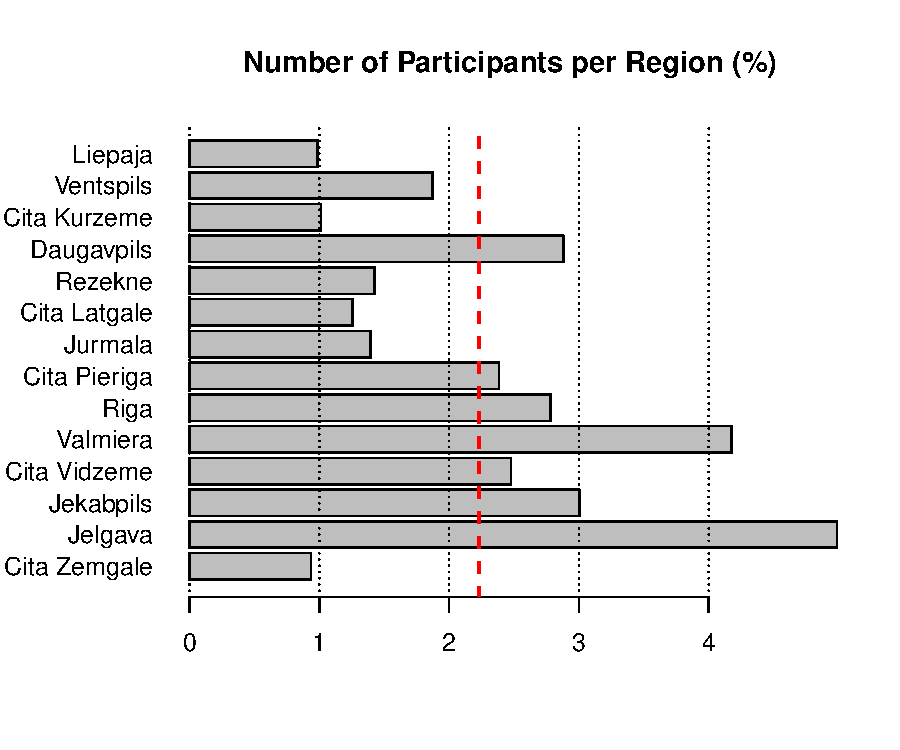
\includegraphics[width=\maxwidth]{figure/minimal-regional-activity-1} 

}



\end{knitrout}


% 1+9+5 aktivitāšu skaitļi pa reģioniem
% Katram no 15 reģioniem dota dzimumu proporcija
%% Stabiņi grupās pa 3 - visi/meitenes/zēni. 

% 1+9+5 aktivitāšu skaitļi pa reģioniem - darbi latviešu valodā
% Katram no 15 reģioniem dota dzimumu proporcija

% 1+9+5 aktivitāšu skaitļi pa reģioniem - darbi krievu valodā
% Katram no 15 reģioniem dota dzimumu proporcija

\subsection{Dalība un sociāli-ekonomiskie rādītāji}

% Trīs 14-bumbulīšu diagrammas

Šeit varētu ievietot diagrammas pa novadiem vai novadu grupām, kas parāda divu parametru attiecību (varētu būt runa par burbulīšu diagrammām, ko zīmē divās dimensijās; turklāt burbulīša laukums ir aptuveni proporcionāls skolēnu skaitam olimpiādē).

\begin{itemize}
\item Sociāli-ekonomisko rādītāju --- bezdarbu, IIN uz 1 iedzīvotāju, pašvaldības izdevumus uz 1 skolēnu vai skolēnu skaitu skolā.
\item Dalībnieku aktivitāti (dalībnieku attiecību pret visiem skolēniem novadā) kā arī olimpiādes summāro rezultātu (punktu summas attiecību pret visiem skolēniem novadā). 
\end{itemize}

Šādas diagrammas palīdzētu saprast, kādi sociālie priekšnoteikumi veicina interesi par olimpiādēm, kāda izglītības politika (piemēram, mazo skolu saglabāšana vai slēgšana; lielāki vai mazāki izdevumi par vienu skolēnu) varētu pozitīvi iespaidot olimpiāžu rezultātus. 

\subsection{Dalībnieku struktūra}



%% Segmenti -- 6 NUTS reģioni
% http://en.wikipedia.org/wiki/Statistical_regions_of_Latvia

Atklātajā matemātikas olimpiādē sastopami darbi latviešu un krievu valodās. Valodu būtu visprecīzāk noteikt, aplūkojot katru konkrēto darbu. Par 41.\ AMO mums šādas informācijas nav, tādēļ valodu secinājām no skolēna re\v{g}istrācijā minētās informācijas, vai arī viņa skolā dominējošo valodu, bet jauktām skolām --- valodu, kas visbiežāk sastopama pieteiktā matemātikas skolotāja audzēkņu vidū. Katras klases joslas iekšpusē iezīmēts balts aplītis, kurš parāda latviešu skolēnu īpatsvaru visu attiecīgās klases audzēkņu vidū. 

Kā redzams, dalība AMO nav pilnīgi proporcionāla latviešu un krievu skolu audzēkņu vidū. Tomēr atšķirības nav lielas --- pie pašreizējās olimpiādes apmeklētības, šo statistiku varētu jūtami izmainīt, papildus piesaistot dalībai olimpiādē dažus desmitus skolēnu. Latvijas vispārizglītojošajās skolās mācības mēdz notikt arī poļu, ukraiņu, baltkrievu, angļu un franču valodās. Šo skolu audzēkņi var izvēlēties rakstīt darbu latviski vai krieviski. Viņu darbi arī pieskaitīti --- atkarībā no re\v{g}istrācijas brīdī izvēlētās valodas.


%% K/L skaita attiecība pa klasēm 
\begin{knitrout}
\definecolor{shadecolor}{rgb}{0.969, 0.969, 0.969}\color{fgcolor}

{\centering 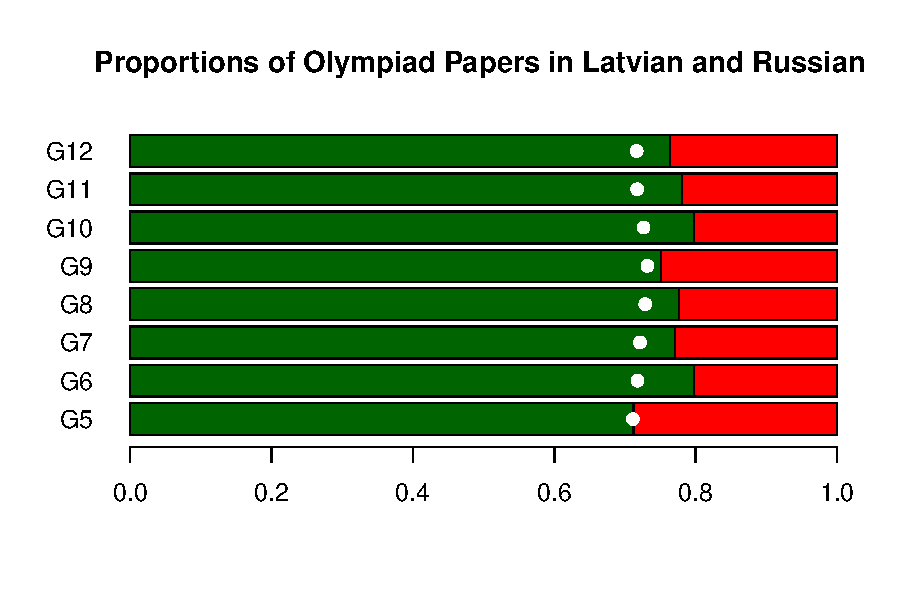
\includegraphics[width=\maxwidth]{figure/minimal-lang-proportions-1} 

}



\end{knitrout}



%% Marimekko diagrammas - dalībnieku dzimumu struktūra pa reģioniem. 
% https://learnr.wordpress.com/2009/03/29/ggplot2_marimekko_mosaic_chart/
%% Segmenti -- 4 urbanizācijas tipi (LV-meitenes, LV-zēni, RU-meitenes, RU-zēni)

Dalībnieku demogrāfisko struktūru var attēlot arī dažādām parametru kombinācijām. Šajā zīmējumā redzams dalībnieku sadalījums pa klasēm (vertikālie stabiņi), un katras klases iekšienē --- arī pa darbu valodām un dalībnieku dzimumiem. Skolēna dzimums re\v{g}istrācijas un rezultātu datos nav dots, 41.\ AMO tos noteicām pēc skolēna vārda. Pasaulē ir zināmas matemātikas sacensības, piemēram, EGMO (European Girls' Mathematical Olympiad), kuru nolūks ir veicināt meiteņu pievēršanos eksaktajām un inženierzinātnēm. Kopš 2013.\ gada EGMO piedalās arī četras vecāko klašu skolnieces no Latvijas.

Latviešu valodā rakstītajiem darbiem zēnu un meiteņu ir aptuveni vienāds skaits, bet krievu valodā rakstītajiem darbiem meiteņu vecāko klašu grupās ir pat divreiz mazāk nekā zēnu.


\begin{knitrout}
\definecolor{shadecolor}{rgb}{0.969, 0.969, 0.969}\color{fgcolor}

{\centering 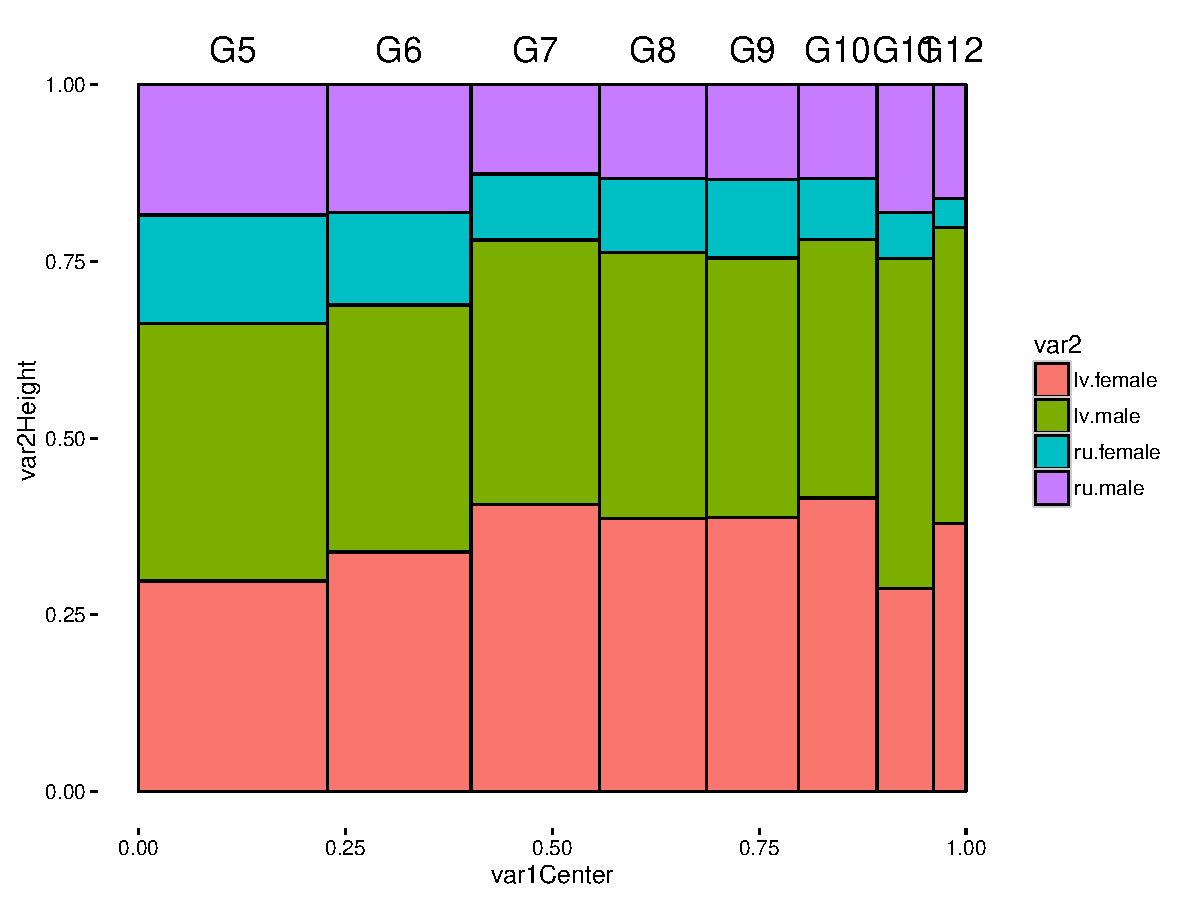
\includegraphics[width=\maxwidth]{figure/minimal-demography-segments-1} 

}



\end{knitrout}





\section{Vidējie rezultāti dalībnieku kategorijām}

Zīmējumā dots rezultātu intervāls katrai klasei. ``Kastītes'' kreisā mala atbilst apakšējai kvartilei, labā mala --- augšējai kvartilei, bet platā zilā svītriņa vidū --- mediānai. Ja klases darbus sakārtotu punktu pieaugšanas secībā un sadalītu četrās vienādās daļās, tad viszemāko punktu ieguvēju ceturtdaļa atrastos uz kreisās ūsas, divas vidējās ceturtdaļas --- kastītes iekšpusē, bet augšējā ceturtdaļa --- uz labās ūsas. Kā redzams attēlā, 12.\ klases skolnieku iegūtais punktu skaits ir būtiski lielāks nekā citu klašu risinātājiem. To varētu izskaidrot daži viegli uzdevumi, kuri ir 12.\ klases komplektā. 

\begin{knitrout}
\definecolor{shadecolor}{rgb}{0.969, 0.969, 0.969}\color{fgcolor}

{\centering 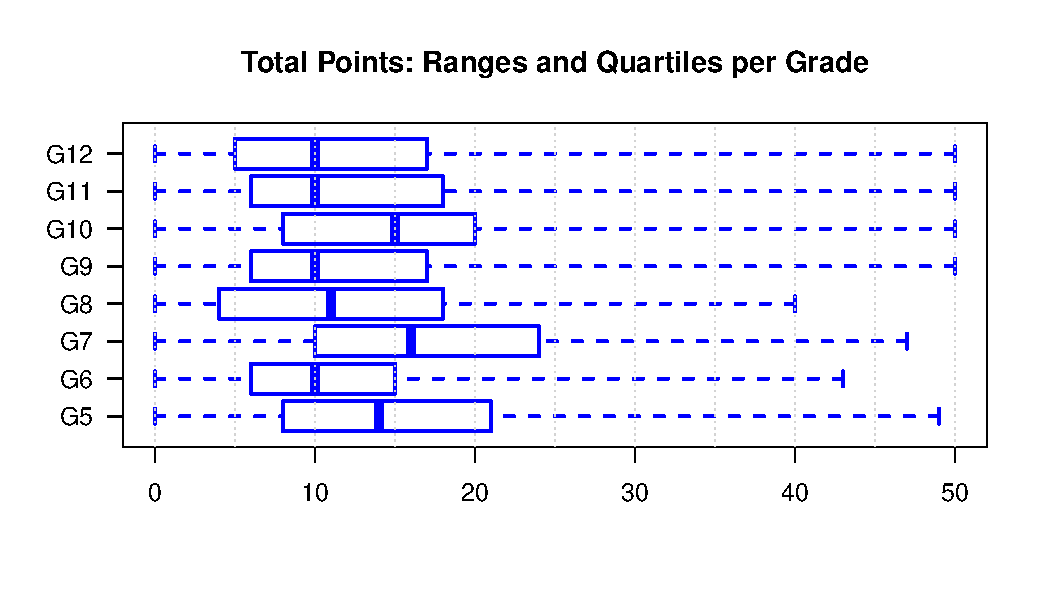
\includegraphics[width=\maxwidth]{figure/minimal-boxplots-per-grade-1} 

}



\end{knitrout}




%% Visu dalībnieku darbi, iekrāsotas godalgotās vietas 
%% Meiteņu un zēnu darbi (Meitenes zīmējam tanī pašā histogrammā)
%% Meitenes ir sazīmētas apakšā. 

%% Urbaniz. tips. Rīgas, 8 lielo pilsētu, mazpilsētu un lauku darbi

%% Latviešu un krievu valodā rakstītie darbi

%% Latviešu un krievu valodā rakstītie darbi -- tikai 9 lielajās pilsētās


\section{Skolas un skolotāji}

% Skolas pēc dalībnieku skaita

% Skolas pēc savāktajiem punktiem

%% Skolotāji pēc dalībnieku skaita

%% Skolotāji pēc savākto punktu skaita

%% Paretto princips pa novadiem; pa skolotājiem utml. Atrast, cik % no skolotājiem nodrošina 80% dalības
%% vai 80% no laureātiem, vai 80% no punktiem. 


\section{Rakstīšanas ilgums un rezultāti}

Daudzās risināšanas telpās dežuranti atzīmēja darba nodošanas laiku. Šeit vizualizējam izplatītākos darbu rakstīšanas ilgumus (nodošanas laiks mīnus 10:30) un dalībnieka rezultāta atkarību no rakstīšanas ilguma.


% Rakstīšanas ilgumu histogramma (15 min. intervāli)


% Vidējais rezultāts atkarībā no rakstīšanas ilguma


% Cik ilgi olimpiādes darbu rakstījuši bērni atkarībā no rezultāta
% 1-3 vietu ieguvēji, atzinību ieguvēji, utt. 


% Cik ilgi olimpiādes darbu rakstījuši bērni atkarībā no dzīvesvietas
% Dalām 14 kategorijās. 


\section{Dati par atsevišķajiem uzdevumiem}

\subsection{Vidējais vērtējums}

Ikviena uzdevuma vērtējums ir skaitlis no 0 līdz 10. Šajā tabulā apkopoti visu uzdevumu vidējie vērtējumi katrā no klašu grupām. 

% Vidējais rezultāts pa uzdevumiem
\begin{knitrout}
\definecolor{shadecolor}{rgb}{0.969, 0.969, 0.969}\color{fgcolor}
\begin{tabular}{l|l|l|l|l|l}
\hline
  & Uzd1 & Uzd2 & Uzd3 & Uzd4 & Uzd5\\
\hline
G5 & 6.70 & 4.72 & 4.21 & 5.25 & 3.06\\
\hline
G6 & 6.35 & 4.41 & 4.02 & 2.96 & 7.27\\
\hline
G7 & 3.52 & 3.98 & 4.98 & 2.77 & 3.89\\
\hline
G8 & 4.44 & 4.91 & 3.70 & 5.32 & 5.41\\
\hline
G9 & 6.64 & 5.00 & 2.29 & 3.72 & 3.79\\
\hline
G10 & 4.53 & 6.12 & 2.71 & 5.31 & 2.09\\
\hline
G11 & 4.23 & 3.20 & 3.08 & 1.75 & 3.88\\
\hline
G12 & 7.09 & 3.61 & 5.38 & 4.17 & 2.57\\
\hline
\end{tabular}


\end{knitrout}

Viszemākais un visaugstākais vidējais vērtējums ir attiecīgi 11.\ klases 4.\ uzdevumam (1.75) un 12.\ klases 1.\ uzdevumam (7.09).

\begin{uzdevums}[11.4]
Doti 99 naturāli skaitļi. Zināms, ka nav tāda skaitļa, ar ko dalītos visi šie skaitļi, un ka jebkuru 50 skaitļu reizinājums dalās ar atlikušo 49 skaitļu reizinājumu. Pierādīt, ka visu 99 skaitļu reizinājums ir naturāla skaitļa kvadrāts. 
\end{uzdevums}


\begin{uzdevums}[12.1]
Atrisināt nevienādību $9^x - 2 \cdot 3^x - 3 \leq 0$.
\end{uzdevums}



% Uzdevumā saņemto punktu daļa dažādu kategoriju dalībnieku rezultātos

% Uzdevuma vērtējuma korelācija ar pārējo uzdevumu summu
\subsection{Uzdevuma vērtējuma korelācija ar pārējo vērtējumu summu}

Ja uzskatām, ka olimpiāde kopumā mēra noteikta veida matemātiskas prasmes, tad par katru uzdevumu var uzdot jautājumu: Cik labi šis uzdevums palīdz mērīt to pašu, ko olimpiādes uzdevumu komplekts kopumā? Ja konkrētais uzdevums labi ``iederas'' starp citiem, tad korelācija būs augsta, ja tas mēra kādas stipri atšķirīgas prasmes nekā citi tās pašas klases uzdevumi, tad korelācija būs mazāka.

Teorētiski varētu gadīties arī negatīva korelācija --- t.i. tāds uzdevums, kuru labākie olimpiādes dalībnieki risināja sliktāk nekā citi. Tad paša uzdevuma vai vērtēšanas sistēmas korektums radītu nopietnas šaubas. Olimpiāžu praksē tomēr negatīvas korelācijas nav vērojamas. Salīdzinoši zemas uzdevuma vērtējuma korelācijas ar citiem uzdevumiem ļauj atrast tos uzdevumus, kuru tēma vai vērtēšanas kritēriji ir būtiski atšķīrušies no citiem uzdevumiem no tā paša 5 uzdevumu komplekta.

\begin{knitrout}
\definecolor{shadecolor}{rgb}{0.969, 0.969, 0.969}\color{fgcolor}
\begin{tabular}{l|l|l|l|l|l}
\hline
  & Uzd1 & Uzd2 & Uzd3 & Uzd4 & Uzd5\\
\hline
G5 & 0.40 & 0.32 & 0.43 & 0.35 & 0.34\\
\hline
G6 & 0.33 & 0.22 & 0.25 & 0.26 & 0.18\\
\hline
G7 & 0.27 & 0.22 & 0.19 & 0.26 & 0.26\\
\hline
G8 & 0.38 & 0.33 & 0.40 & 0.32 & 0.24\\
\hline
G9 & 0.34 & 0.26 & 0.27 & 0.26 & 0.28\\
\hline
G10 & 0.31 & 0.13 & 0.16 & 0.30 & 0.14\\
\hline
G11 & 0.40 & 0.24 & 0.37 & 0.33 & 0.36\\
\hline
G12 & 0.18 & 0.14 & 0.16 & 0.05 & 0.31\\
\hline
\end{tabular}


\end{knitrout}

Mazākās korelācijas ar citiem tās pašas klases uzdevumiem ir 10.\ klases 2.\ uzdevumam (0.13) un 12.\ klases 4.\ uzdevumam (0.05). 

\begin{uzdevums}[10.2]
Dotas divas paralēlas taisnes. Uz vienas no tām atzīmēti 14 zaļi punkti, uz otras -- 14 sarkani punkti. Kādu lielāko skaitu nogriežņu, kuriem viens galapunkts ir zaļš, bet otrs -- sarkans, var novilkt tā, lai tie nekrustotos? Saka, ka nogriežņi krustojas, ja tiem ir kopīgs iekšējais punkts, t.i., ja tiem ir kopīgs tikai galapunkts, tie nekrustojas.
\end{uzdevums}


\begin{uzdevums}[12.4]
Vai kvadrātu ar malas garumu 10 var noklāt ar 25 ``krustiņiem'' (skat. zīm.), kuri sastāv no 5 kvadrātiem ar malas garumu 1? ``Krustiņi'' drīkst pārklāties, kā arī iziet ārpus dotā kvadrāta malām.\\

\includegraphics[width=20mm]{pentomino-x.png}
\end{uzdevums}



\end{document}
